\starthis\section[球型势阱]{球型势阱} \label{sec:05.03} % 
% \makebox[5em][s]{} % 短题目拉间距

{\heiti 1. 无限深球形势阱}

设粒子被无限深球形势阱
\begin{empheq}{equation}\label{eq53.1}
	{V(r)=}
	\begin{dcases}
		0,\quad r<a	\\
		\infty,\quad r\geqslant a
	\end{dcases}
\end{empheq}
限制在球内$(r<a)$运动.球内薛定谔方程与自由粒子相同,球外边界条件为
\begin{empheq}{equation}\label{eq53.2}
	r\geqslant a,\quad \varPsi=0
\end{empheq}
由于是中心力场,轨道角动址$\boldsymbol{L}$是守恒量,$(\hat{H},\hat{\boldsymbol{L}}^{2},\hat{L}_{z})$的共同本征函数可以表示成(略去归一化常数)
\begin{empheq}{equation}\label{eq53.3}
	\varPsi(r,\theta,\varphi)=j_{l}(kr)Y_{lm}(\theta,\varphi),\quad r<a
\end{empheq}
其中
\begin{empheq}{equation}\label{eq53.4}
	k=\frac{\sqrt{2\mu E}}{\hbar}
\end{empheq}
边界条件\eqref{eq53.2}具体表现为
\begin{empheq}{equation}\label{eq53.5}
	j_{l}(ka)=0
\end{empheq}
这也就是决定能级的条件.$j_{l}(x)$的零点记成$x_{nl}$($n=1,2,\cdots$是零点的序数),其值可以从贝塞耳函数表查得,如表\ref{lab.5-1}.$k$和$E$的特征值由$x_{nl}$决定,
\begin{empheq}{equation}\label{eq53.6}
	k_{nl}=\frac{x_{nl}}{a}
\end{empheq}
\begin{empheq}{equation}\label{eq53.7}
	E_{nl}=\frac{\hbar^{2}}{2\mu}k_{nl}^{2}=\frac{\hbar^{2}}{2\mu a^{2}}x_{nl}^{2}
\end{empheq}
由于各$j_{l}$没有相同的零点,因此属于$l=0,1,2\cdots$的各组能级互不相同.能级$E_{nl}$的简并度等于$(2l+1)$,相应于$(2l+1)$种$m$值,
\begin{empheq}{equation*}
	m=0,\pm1,\pm2,\cdots,\pm l
\end{empheq}
按照光谱学的习惯,各$l$值用字母表记:

\begin{empheq}{alignat*=7}
	l &\quad 0 &\quad 1 &\quad 2 &\quad 3 &\quad 4 &\quad 5	\\
	\text{字母} &\quad s &\quad p &\quad d &\quad f &\quad g &\quad h	\\
\end{empheq}
能级$E_{10}$已成$1\si{s}$,$E_{23}$记成$2\si{f}$,等等.

\begin{table}[!h]
	\begin{center}
		\caption{$\dfrac{x_{nl}}{\pi}$的数值}\label{lab.5-1}
		\setlength{\tabcolsep}{4mm}	% 调节表格尺寸
		%\resizebox{h-length}{v-length}{text}
		\begin{tabular}{c|c|c|c|c|c}
			\hline 
			\diagbox{$l$}{$n$} & 1 & 2 & 3 & 4 & 5	\\	\hline
			0 & 1 & 2 & 3 & 4 & 5	\\	\hline
			1 & 1.4303 & 2.4590 & 3.4709 & 4.4774 & 5.4816	\\	\hline
			2 & 1.8346 & 2.8950 & 3.9225 & 4.9386 & 5.9489	\\	\hline
			3 & 2.2243 & 3.3159 & 4.3602 & 5.3870 & 6.4050	\\	\hline
			4 & 2.6046 & 3.7258 & 4.7873 & 5.8255 & 6.8518	\\	\hline
			5 & 2.9780 & 4.1274 & 5.2059 & 6.2558 & 7.2908	\\	\hline
			6 & 3.3464 & 4.5224 & 5.6176 & 6.6793 & 7.7231	\\	\hline
		\end{tabular}
	\end{center}
\end{table}

由表\ref{lab.5-1}可以看出,能级由低到高的次序(即$x_{nl}$的次序)是
\begin{empheq}{equation*}
	1\si{s},1\si{p},1\si{d},2\si{s},1\si{f},2\si{p},1\si{g},2\si{d},1\si{h},3\si{s},2\si{f},\cdots
\end{empheq}

s态$(l=0)$的能级条件是
\begin{empheq}{equation*}
	j_{0}(x)=\frac{\sin x}{x}=0,\quad x=ka
\end{empheq}
解为
\begin{empheq}{align}\label{eq53.8}
	x_{n0}&=n\pi,\quad n=1,2,3,\cdots	\nonumber\\
	k_{n0}&=\frac{n\pi}{a},\quad E_{n0}=n^{2}\frac{\pi^{2}\hbar^{2}}{2\mu a^{2}}
\end{empheq}
这结果与一维无限深势阱相同,原因是,$l=0$时离心势能为0,$u(r)=n\varPsi$所满足的径向方程以及边界条件均类似于一维无限深势阱问题.基态能级是
\begin{empheq}{equation}\label{eq53.9}
	E_{10}=\frac{\pi^{2}\hbar^{2}}{2\mu a^{2}}
\end{empheq}
\eqref{eq53.7}式也可以写成
\begin{empheq}{equation*}\label{eq53.7'}
	E_{nl}=\bigg(\frac{x_{nl}}{\pi}\bigg)E_{10}
	\tag{$5.3.7^{\prime}$}
\end{empheq}
由表\ref{lab.5-1}可见,能级分布不是等距离的,但最低的几个能级分布比较均匀.高激发态的情况就大不一样.根据$j_{l}$的渐近公式[\eqref{eq52.18}式]易见其零点约为
\begin{empheq}{equation}\label{eq53.10}
	x_{nl}\approx \bigg(n+\frac{l}{2}\bigg)\pi
\end{empheq}
[当$n>l$,\eqref{eq53.10}式的近似程度就相当好,参看表\ref{lab.5-1}]因此
\begin{empheq}{equation*}
	x_{nl}\approx x_{n+1,l-2}\approx x_{n+2,l-4}\approx \cdots
\end{empheq}
能级出现近似简并的微妙情形.这种近似简并在$n<l$时也偶尔出现,如$E_{15}$和$E_{30}$,$E_{23}$和$E_{16}$,$E_{17}$和$E_{24}$,等等.

{\heiti 2.氘核}

氘核是质子和中子在核力(强作用)作用下形成的束缚态,而且是唯一的束缚态.根据实验测定,氘核的结合能为$|E|=\num{2.237}\si{MeV}$.

\begin{wrapfigure}[9]{r}{7em}
	\centering
	\small
	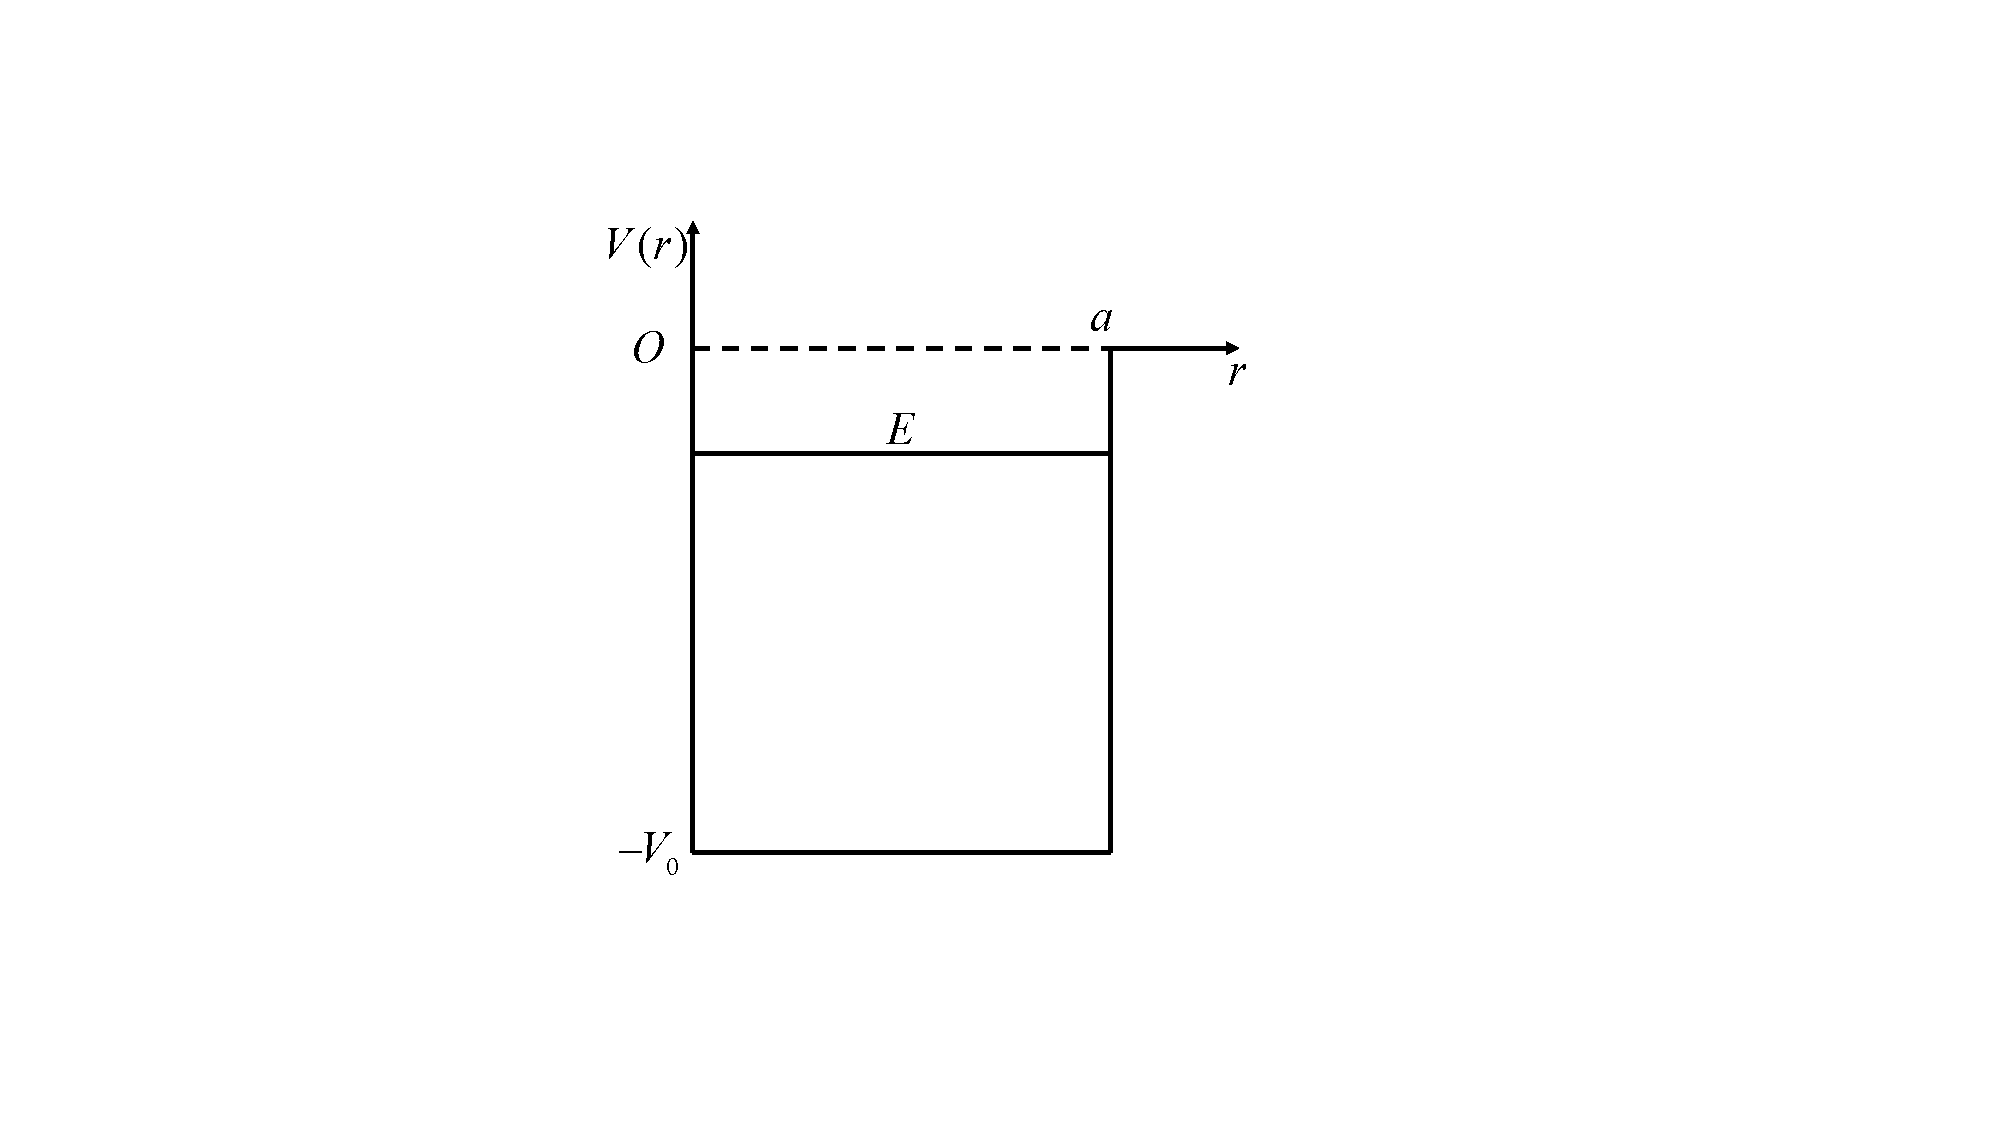
\includegraphics[width=3cm]{QM file/figure/5-3}
	\caption{}\label{fig.5-3}
\end{wrapfigure}
核力是短程力,力程约2\si{fm},作用强度约$20\sim 30 \si{MeV}$,近似地可以用图\ref{fig.5-3}所示的球形势阱表示质子-中子之间的核力作用势,
\eqlong
\begin{empheq}{equation}\label{eq53.11}
	{V(r)=}
	\begin{dcases}
		-V_{0},\quad r\leqslant a	\\
		0,\quad r>a
	\end{dcases}
\end{empheq}\eqshort
$a$为力程,$V_{0}$为作用强度.利用结合能的实验值可以求出$V_{0}$与$a$的依赖关系,如下.

氘核是稳定的,相当于基态,角量子数$l=0$,波函数可以写成(不考虑归一化)
\begin{empheq}{equation}\label{eq53.12}
	\varPsi(r)=\frac{u(r)}{r}
\end{empheq}\eqnormal
$u(r)$满足径向方程[\eqref{eq51.14}式,$l=0$]
\begin{empheq}{equation}\label{eq53.13}
	\bigg[-\frac{\hbar^{2}}{2\mu}\frac{d^{2}}{dr^{2}}+V(r)-E\bigg]u(r)=0
\end{empheq}
亦即
\begin{empheq}{equation*}\label{eq53.13'}
	{}
	\begin{dcases}
		\frac{d^{2}}{dr^{2}}u+k^{2}u=0,\quad r\leqslant a	\\
		\frac{d^{2}}{dr^{2}}u-\beta^{2}u=0,\quad r>a
	\end{dcases}
	\tag{$5.3.13^{\prime}$}
\end{empheq}
其中
\begin{empheq}{equation}\label{eq53.14}
	k=\frac{\sqrt{2\mu(V_{0}+E)}}{\hbar},\quad \beta=\frac{\sqrt{-2\mu E}}{\hbar}(E<0)
\end{empheq}
边界条件为
\begin{empheq}{equation}\label{eq53.15}
	r\rightarrow 0,\quad u\rightarrow 0;\quad r\rightarrow \infty,\quad u\rightarrow 0
\end{empheq}
\eqref{eq53.13'}式满足这边界条件的解为
\begin{empheq}{equation}\label{eq53.16}
	{u(r)=}
	\begin{dcases}
		\sin kr,\quad r\leqslant a	\\
		Ce^{-\beta r}, \quad r>a
	\end{dcases}
\end{empheq}
$r=a$处,$\frac{u^{\prime}}{u}$应该连续,由此求得能级公式
\begin{empheq}{equation}\label{eq53.17}
	\cot ka=-\frac{\beta}{k}
\end{empheq}
这公式类似于一维方势阱奇宇称态的能级公式,上式等价于
\begin{empheq}{equation}\label{eq53.18}
	\sin^{2}ka=\frac{k^{2}}{k^{2}+\beta^{2}}=1+\frac{E}{V_{0}}
\end{empheq}
对于氘核,$E=-\num{2.237}\si{MeV}$,$\mu$应该取为质子-中子体系的约化质量,
\begin{empheq}{align}\label{eq53.19}
	\mu=&\frac{m_{0}m_{p}}{m_{n}+m_{p}}\approx\frac{m_{p}}{2},\quad 2\mu c^{2}\approx 938\si{MeV}	\nonumber\\
	k^{2}&=\frac{2\mu(V_{0}+E)}{\hbar^{2}}=\frac{2\mu c^{2}(V_{0}+E)}{\hbar^{2}c^{2}}
\end{empheq}
\begin{table}[!h]
	\begin{center}
		\caption{}\label{lab.5-2}
		\setlength{\tabcolsep}{8mm}	% 调节表格尺寸
		%\resizebox{h-length}{v-length}{text}
		\begin{tabular}{c|c|c|c}
			\hline 
			$V_{0}/$\si{MeV} & 30 & 25 & 20 	\\	\hline
			$a/$\si{fm} & 2.26 & 2.53 & 2.92 	\\	\hline
		\end{tabular}
	\end{center}
\end{table}
在\eqref{eq53.18}、\eqref{eq53.19}式中,取实验值$E=\num{-2.237} \si{MeV}$,再指定一个$V_{0}$值,由\eqref{eq53.19}式算出$k$,由\eqref{eq53.18}式算出$ka$,从而求出与$V_{0}$相应的$a$值.结果如表\ref{lab.5-2}.

其中前二组数据比较接近于用其他方法(例如散射实验)确定的数值.




